\section{Kings: The Tr\'ebuchet and When It Is Exact}\label{sec:kings}

In chess a player with no pawn move would move the king, or be stalemated, a draw. The tr\'ebuchet removes
stalemate: a side with no pawn move must move a king, and loses. We now ask when this gives the true chess result. Our king-and-pawn solver plays
real chess, with en passant, stalemate and any of the four promotions, but no fifty-move rule; an independent
reference solver, written from the rules alone, agrees with it on all $1{,}418{,}480$ positions of its test runs
\lab{C2}. Our solver's results below are \lab{C1} unless a second program or the Lichess
tablebase~\cite{LichessTB} confirms them.

\begin{figure}[!t]
\centering
\begin{subfigure}{0.32\columnwidth}
\centering
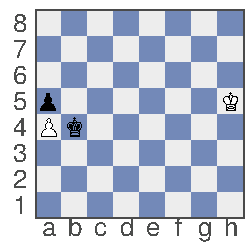
\includegraphics[width=\linewidth]{figures/trebuchet_2025.pdf}
\caption{\pos{W~Kh5~a4 / \mbox{B~Kb4~a5}}}
\label{fig:trebuchet_2025}
\end{subfigure}\hfill
\begin{subfigure}{0.32\columnwidth}
\centering
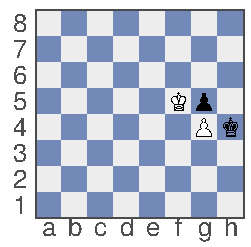
\includegraphics[width=\linewidth]{figures/trebuchet.pdf}
\caption{\pos{W~Kf5~g4 / \mbox{B~Kh4~g5}}}
\label{fig:trebuchet}
\end{subfigure}\hfill
\begin{subfigure}{0.32\columnwidth}
\centering
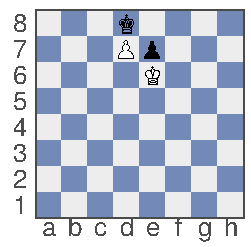
\includegraphics[width=\linewidth]{figures/kinggroup72.pdf}
\caption{\pos{W~Ke6~d7 / \mbox{B~Kd8~e7}}}
\label{fig:kinggroup72}
\end{subfigure}
\caption{King groups: (a) a tr\'ebuchet on the cylinder (files a and h adjacent) and (b) the tr\'ebuchet T
(ordinary board), both real mutual zugzwangs, $0$ when alone; (c) a king group from the 2025 study (cylinder;
Section~\ref{sec:sums}) that does not count as $0$: it draws with white to move, a zugzwang for black only.}
\label{fig:kings}
\end{figure}

In Fig.~\ref{fig:trebuchet_2025} only the kings can move. White to move must give up a4, since the only square
next to a4 that the king on h5 can move to, h4, is attacked by the a5 pawn across the seam; black to move loses
a5 in the same way. So this is a real mutual zugzwang that exists only because of the seam \lab{C2}.
Fig.~\ref{fig:trebuchet} shows the same idea on files f to h of the ordinary board; the Lichess tablebase
confirms that it is a mutual zugzwang \lab{C2}. We call this group T and place it beside every ordinary-board
pawn position in this paper.

\subsection{When Is the Frozen Tr\'ebuchet Exact?}\label{sec:kings-valid}

A \emph{king group} $Z$ is the two kings and some pawns on a block of files whose neighboring files, the
\emph{buffer}, hold no pawns; a \emph{decisive event} is a move in $Z$ or one creating a passed pawn.

\begin{theorem}[Validity of the convention; \lab{S}]\label{thm:validity}
Let a position consist of pawn components and a king group $Z$ with its buffer, let $X$, the position without $Z$, have no passed pawn, and suppose that before the
first decisive event:
\begin{enumerate}
\item[(V1)] outside $Z$ the legal chess moves are exactly the model's pawn moves, with the same results (en
  passant included); none gives check, nobody is in check, and the side to move has a legal move (one in $Z$
  counts);
\item[(V2)] in chess, the side that gets a passed pawn wins, and a race is won as the race rule says;
\item[(V3)] in chess, every move in $Z$ loses (it is \emph{decisively punished}).
\end{enumerate}
Then the chess result, with either side to move, is the outcome of $W(X)$, the pawn game that ends at the first
passed pawn (Section~\ref{sec:sums-hss}), without draws.
\end{theorem}

\begin{proof}[Proof sketch]
By (V3) neither side moves in $Z$ without losing, so until the first decisive event both play the pawn game;
by (V1) the side to move always has a legal move, a pawn move or a move in $Z$; the pawn game is finite, so some
decisive event occurs, and by (V2) and (V3) that event decides the chess game as it decides $W(X)$. The full
proof is in Section~S12.
\end{proof}

\begin{corollary}[\lab{S}]\label{cor:v4}
If also (V4) $X$ is hereditarily sum-safe (Definition~\ref{def:hss}) and satisfies condition (E) of
Theorem~\ref{thm:hss}, and $\BIG$ exceeds the number of moves either side can make, the chess result is
the outcome class of the components' $\pm\BIG$ value.
\end{corollary}

\begin{proof}
By Theorem~\ref{thm:validity} the chess result is the outcome of $W(X)$, and by Theorem~\ref{thm:hss} this is
the outcome of $S(X)$ (Section~\ref{sec:sums-hss}).
\end{proof}

Each condition can fail: a stalemate trap leaves the loser without a move (V1), a passed pawn does not win its
race (V2), a king walks over to the pawns or, in Fig.~\ref{fig:kinggroup72}, white's king moves go unpunished
(V3), and a $+\BIG$ cancels a $-\BIG$ (V4). For (V3) there is a local test: a move in $Z$ has a
\emph{certificate of horizon $h$} if, with only $Z$ on the board, the punisher promotes or mates within $h$
moves of its reply, no defender pawn outside $Z$ is that fast, and no stalemate comes first. In the \emph{promotion game} (the first
promotion wins) such a move loses for its mover \lab{S}; in chess even wider margins can fail. The exact clauses and the proof are in Section~S12; a local test for (V2)
and the loopy games of kings with spare moves are in Section~S2.

\subsection{How Often Does the Convention Fail?}\label{sec:kings-sweep}

We solved, with the kings played out, every component with at most two pawns a side beside a tr\'ebuchet on
boards with six ranks (one file of the six-file cylinder and of the five-file ordinary board, files d and e of
the seven-file cylinder; queen promotions only, at most two). Of these, $500$ start without a race and have a
determined result. Under the textbook test, $159$ of the $500$ get the wrong outcome \lab{C1}: $107$ through
the kings alone, $18$ through en passant and $34$ because a passed pawn does not win its race. The e.p.-aware
test repairs the $18$ e.p.\ failures, but the kings undo $13$ of these repairs. In each race failure a blocked
enemy pawn steps level with its blocker and promotes first. Ending the game only at a passer
that wins the race by the square rule removes all $52$ convention failures with frozen kings; with real kings
$31$ stay repaired, which leaves $128$ mismatches, all from the kings \lab{C1}. The rule is not sound on every
board (Section~S16). Of the $2{,}154$ $8\times8$ positions beside a tr\'ebuchet whose real results we know, $105$ are
draws; in the other $2{,}049$ the model names the winner in $92.5\%$, against $83\%$ and $84\%$ under the mover
and opponent rules \lab{C1} (Section~S2).
